% #############################################################################
%															Hinderniskarte und Lokalisierung
% #############################################################################
\chapter{Hinderniskarte und Lokalisierung}
\label{lokalisierung_cha}
% ********************************************************************************
% 										Aufgabenstellung
% ********************************************************************************
\section{Aufgabenstellung}
\label{lokalisierung_aufgabenstellung_sec}
\authorsection{\editorandreas}
% -----------------------------------------------------------------------------
%													Lokalisierung
\subsection{Lokalisierung}
Die Aufgabe der Lokalisierung, im Kontext der Robotik, ist die Bestimmung der
Roboter Pose, welche die Position und Orientierung des Roboters in seiner Umgebung vollständig beschreibt.
 Um Bahnplanung und Steuerung zu ermöglichen muss die Pose des Roboters bekannt sein,
 damit sich dieser gefahrlos fortbewegen und sicher mit der Umwelt interagieren kann.
 Für einen Menschen ist die Lokalisierung selbstverständlich, für einen Roboter
 stellt sie allerdings eine Herausforderung dar.
 Aufgrund einer unbekannter Startposition oder von Messungenauigkeiten während
 der Fortbewegung, kann die Pose eines Roboters nur in den seltensten Fällen
 genau bestimmt werden.
  Von lokaler Lokalisierung wird gesprochen wenn die aktuelle Pose des Roboters
 in seiner Umwelt bekannt ist und bei einer Positionsänderung des Roboters
 fortlaufend aktualisiert wird um sie auf dem neusten Stand zu halten. Hier
 werden Schätzungen der Bewegung aufgrund der Odometrie Sensorik mit Hilfe von weiteren Daten zur Posenbestimmung korrigiert. Dieses Vorgehen soll eine Aufsummierung von Fehlern bei der
 Schätzung der Bewegung durch die Odometrie verhindern. Im Gegensatz dazu ist
 bei der globalen Lokalisierung die aktuelle Pose des Roboters in seiner Umwelt
 nicht bekannt und muss zum Beispiel anhand von Kartenmaterial geschätzt werden.
 Man sieht leicht ein, dass bei dieser Art der Lokalisierung die Initiale
 Schätzung einen beliebig großen Fehler aufweisen kann.
 Nach dieser Einführung sollte klar geworden sein das es notwendig
 ist eine Lokalisierung durchzuführen um es unserem Roboter zu
 ermöglichen sich fortzubewegen.
% -----------------------------------------------------------------------------
%													Hinderniskarte
\subsection{Hinderniskarte}
Abgesehen von der Lokalisierung gibt es noch einen weiteren Grund warum es für einen mobilen Roboter unumgänglich ist,
 dass eine interne Repräsentation seiner Umgebung existiert. Karten, die zur Lokalisierung eingesetzt werden,
 enthalten meist nicht alle statischen Hindernisse, da diese Karten zu einem gewissen Zeitpunkt erstellt wurden und
 in der Zwischenzeit wahrscheinlich neue Objekte hinzugekommen oder bereits Vorhandene versetzt worden sind.
 Außerdem enthalten solche Karten offensichtlich keine Hindernisse die sich bewegen können, wie beispielsweise Menschen.
 Ein Hindernis ist ganz allgemein ein Bereich der von dem Roboter nicht befahren werden kann. Eine Darstellung der Hindernisse
 relativ zur Roboterpose wird als Hinderniskarte bezeichnet. Eine solche Karte
 kann zum Beispiel mit Hilfe von Laser- oder Kameradaten erstellt werden.
 Eine Kombination des Materials mehrerer Sensoren ist normalerweise das Sinnvollste,
 da Laser beispielsweise keine negativen Hindernisse erkennen können.
 Als negative Hindernisse werden Bereiche bezeichnet die im Vergleich zur
 gegenwärtigen Position eine geringere Höhe aufweisen.
 Ein Beispiel für ein solches Hindernis ist eine Treppe in ein tiefer gelegenes
 Stockwerk. Das erstellen einer Hinderniskarte ist aus den oben genannten
 Gründen essentiell um eine Bahnplanung für einen mobilen Roboter
 durchführen zu können.
% -----------------------------------------------------------------------------
%													Virtual protective Field
\subsection{Virtual protective Field}
Die Aufgabe der Bahnplanung besteht darin auf Grundlage der Lokalisierung und der Hinderniskarte einen Weg zu einer
 bestimmten Position zu finden. Danach wird dieser Weg vom Roboter abgefahren. Allerdings kann es während dem Abfahren der gefundenen
 Route Aufgrund eines Hindernisses, dass sich in den Weg des Roboters bewegt bevor erneut geplant werden kann oder
 schlicht Aufgrund eines Fehlers in der Planung dazu kommen, dass der Roboter mit einem Hindernis kollidiert.
 Daher wird eine Möglichkeit benötigt auf einer tieferen Ebene wie der Bahnplanung das unbeabsichtigte kollidieren mit einem Hindernis
 zu verhindern. An dieser Stelle kommt das sogenannte „Virtual protective Field“ ins Spiel, von welchem ein Bereich um den Roboter auf
 Hindernisse überprüft und beim Auffinden eines Solchen ein Signal erzeugt wird, damit der Roboter gestoppt werden kann bevor er
 auf das Hindernis trifft. Dieser Bereich muss mit der Geschwindigkeit des
 Roboters wachsen bzw. schrumpfen so das sichergestellt ist, dass auf jeden
 Fall eine Kollision verhindert werden kann.
% ********************************************************************************
% 										Grundlagen Lokalisierung
% ********************************************************************************
\section{Grundlagen Lokalisierung}
\label{lokalisierung_grundlagen_sec}
\authorsection{\editordummy}
\todo[inline]{Lokalisierungs-Gruppe: Schreiben}
% -----------------------------------------------------------------------------
%													Lokalisierung
\subsection{Lokalisierung}
Nachdem wir im vorigen Abschnitt neben einer kurzen Erläuterung der
Materie hauptsächlich die Aufgaben und deren Ziele betrachtet haben,
 wollen wir hier eine detaillierte Betrachtung der Möglichkeiten
 und Verfahren zur Positionsbestimmung durchführen.
 
\subsubsection{Odometrie}
Ein einfacher Ansatz zur Positionsbestimmung ist die Verwendung
 von Schrittzählern, welche die Bewegung der Roboterräder oder
 -Beine misst. Über eine Umrechnungsfunktion (meist: lineare
 Abbildung) lässt sich aus der Anzahl der zurückgelegten Schritte
 eine Pose relativ zur Ausgangspose berechnen.

\begin{itemize}
  \item Vorteile:
  \begin{itemize}
    \item Relativ Stör-unanfällig unter Normalbedingungen\\ 
    (Ausnahmen: glatter, weicher, unebener Untergrund)
    \item Vernachlässigbarer Rechenaufwand
    \item Vernachlässigbarer Implementations-Aufwand
  \end{itemize}
  \item Nachteile:
  \begin{itemize}
    \item Offset-Fehler steigt linear mit dem Betrag der Schrittzahl
    \item Ursprungsposition muss bekannt sein (vorgegeben werden)
    \item Fehler abhängig vom Untergrund
    \item Bei auf Schlupf basierenden (omnidirektionalen)
     Plattformen Fehler höher
   \end{itemize}
\end{itemize}

\subsubsection{Kartenbasierte Lokalisierung}

Anhand von gegebenem Kartenmaterial kann aus einem Sensorbild
 der Umgebung die Position des Roboter geschätzt werden.
 Dazu werden zum Beispiel markante Punkte aus dem Sensorbild mit den
 Daten des Kartenmaterials abgeglichen. Im bestmöglichen Fall
 existiert nur eine mögliche Übereinstimmung, anhand derer der
 Roboter seine eigene Position bestimmen kann.

\begin{itemize}
  \item Vorteile:
  \begin{itemize}
    \item Keine Fehlerakkumulation über Zeitverlauf
    \item Keine Ursprungsposition notwendig
  \end{itemize}
  \item Nachteile:
  \begin{itemize}
    \item Störanfällig (spiegelnde Oberflächen, bewegende Objekte)
    \item Benötigt aktuelles Kartenmaterial
    \item hoher Rechenaufwand
    \item hoher Implementierungs-Aufwand
   \end{itemize}
\end{itemize}

\subsubsection{Landmarkbasierte Lokalisierung}

In einer bekannten Umgebung können Landmarks (QR-Codes, Bodenlinien,
 GPS-Satelliten) angebracht werden. Diese können durch Sensoren
 am Roboter wiedererkannt werden und ermöglichen die Lokalisierung
 z.B. mittels Triangulierung.

\begin{itemize}
  \item Vorteile:
  \begin{itemize}
    \item (durchschnittlicher) Fehler niedrig
    \item Zuverlässig (max. Fehler niedrig)
    \item Keine Fehlerakkumulation über Zeitverlauf
  \end{itemize}
  \item Nachteile:
  \begin{itemize}
    \item Landmarks notwendig
    \item Landmarks müssen von überall sichtbar sein
    \item Kartenmaterial u.U. notwendig
   \end{itemize}
\end{itemize}

Um die Nachteile der verschiedenen Lokalisierungsmethoden zu
 verringern werden in der Regel mindestens zwei Methoden miteinander
 kombiniert. Aufgrund der einfachen Implementierung und der geringen
 Störanfälligkeit ist meistens die Odometrie in Kombination mit
 anderen Systemen vorzufinden. Bei Verwendung mehrerer Methoden sind
 dementsprechend viele fehlerbehaftete Annahmen der aktuellen
 Roboterpose gegeben. Im Folgenden wollen wir zwei unterschiedliche
 Verfahren vorstellen, welche aus diesen Annahmen bestmöglich die
 aktuelle Roboterpose bestimmen.
 
\subsubsection{Kalman-Filter}
  Ein Verfahren, um den gesamten Fehler zu minimieren ist das
  Kalman-Filter.
\todo[inline]{Kurze Erläuterung / Einführung in das
Kalman-Filter}
\subsubsection{Partikel-Filter}
\todo[inline]{Kurze Erläuterung / Einführung in den
 Partikel Filter}
 
% ********************************************************************************
% 										Umsetzung
% ********************************************************************************
\section{Umsetzung}
\label{lokalisierung_umsetzung_sec}
\authorsection{\editordummy}
% -----------------------------------------------------------------------------
%													Lokalisierung
\subsection{Lokalisierung} 
In diesem Abschnitt wollen wir uns mit der eigentlichen Umsetzung der
 Lokalisierung beschäftigen. Wie sie wahrscheinlich schon aus Kapitel
 \ref{grundlagen_cha} wissen, verfügen die beiden Roboter HoLLiE und
 Odete über sehr ähnliche Sensoren, die zur Lokalisierung verwendet werden
 können. Der Roboter, Odete weist 2 Winkelencoder (in Segway
 Omni\todoprivate{in Wirklichkeit ? eventuell schon in Grundlagen besprochen
 dann hier unnötig}) und ein 270 Grad Sick Laserscanner (Scheibenförmiger Scan)
 auf.
 HoLLiE verfügt über ?\todoprivate{in Wirklichkeit ?} Winkelencoder und zwei
 ?\todoprivate{in Wirklichkeit ?} Grad Sick Laserscanner. Offensichtlich musste,
 um ein sicheres Fortbewegen des Roboters zu gewährleisten, für das Odete Projekt
 ebenfalls eine Lokalisierung implementiert werden.
 Im Folgenden wollen wir kurz auf die Idee bei der Wahl der Gruppen
 und Module für die Lokalisierung im Odete Projekt eingehen.
 Die verwendete MCA2 Struktur der Odete basiert auf einem bestimmten Paradigma.
 Ziel ist es eine hohe Flexibilität zu erreichen. Sensoren und Plattformen sollen
 beliebig kombinierbar sein. Wir entschieden uns daher dazu diese Struktur auch
 beim Segway Omni Projekt weiterzuführen. Dadurch konnten alte Programmstrukturen
 übernommen und/oder adaptiert und außerdem dieselbe Flexibilität wie im Odete Projekt
 erreicht werden. Daher gelten die folgenden Erläuterungen zur Lokalisierung
 auch fast uneingeschränkt für beide Robotersysteme.
 Zur Positionsschätzung wir bei beiden Systemen eine Kombination aus kartenbasierter Lokalisierung
 und Odometrie verwendet. Die Schätzwerte aus beiden Messungen werden mit einem Kalman-Filter zu einer
 Synthese geschätzt. Dem Kalman-Filter ist eine Queue (FIFO) vorgeschaltet, in der jede Schätzung
 mit einem Timestamp registriert wird. So können die Messwerte in zeitlich korrekter Reihenfolge
 eingerechnet werden, selbst dann, wenn sie nach der Verarbeitung in einer anderen Reihenfolge
 im Kalman-Filter registriert werden. Die für die Odometrie benötigte Winkelschrittmessung der Räder wird direkt
 von der Segway-Antriebsplattform geliefert.
 Es wird angenommen, dass der Fehler linear ansteigt mit der durch den Reifen zurückgelegten Strecke.
 Falls eine gute Schätzung aus der kartenbasierten Lokalisierung in den Kalman-Filter übergeben wird,
 wird die Pose korrigiert und der Odometriefehler wieder gesenkt.



\todo[inline]{Geplanter Aufbau -> Grundlegende Idee für die Umsetzung
 --- Bild der Gruppe, erläutern der Funktion der Module}
 \todo[inline]{Stuktur des Materials an die gewünschte form anpassen etwa
 durch:die aussagen zur lokalisierung gelten generell für hollie und sowie da
 bla bla und dann die ganzen erklärungen}


Im bereits bestehenden Odete Projekt wurde die Lokalisierung mit Hilfe von Odometrie und Laserdaten durchgeführt. 


Die Verarbeitung der Odometrie und die anschließende Korrektur durch die Kombination mit den
 Laserdaten XXmit hilfeXX eines Kalmanfilters fand in der Hal Gruppe (Hardwar Abstraction Layer)
 und die Verarbeitung der Laserdaten in der Sal Gruppe (Scanner Abstraction Layer) statt.
 Eine ähnliche Hal Gruppe existiert in der uns zur Verfügung gestellten Projektstruktur Segway Omni.
 Nach einer Unterredung mit unserem Betreuer Jan Oberländer bekamen wir auch einige Zeit danach eine
  ähnliche Sal Gruppe zur Vorverarbeitung und Simulation der Laserdaten der angebrachten Sickscanner. 


Hardware Abstraction Layer (Hal) und (später) Scanner Abstraction Layer (Sal)
aus dem bereits bestehenden Segway Omni Projekt


Adaption der Vorhanden Gruppen und Module zur Lokalisierung 
Anpassung von LLSP, HLSP, Hal \& Sal an das Segway Omni Projekt
Erweiterung auf beliebige Menge von Scannern


Parametrisierung über Multiplexer und XML-Config-File ermöglichen
Parameter anpassen auf neue Sensor-Anordnung



Kartenbasierte Lokalisierung

Eine kartenbasierte Posen-Schätzung wird in folgenden Schritten ermittelt.

    Scheibenförmiger Laser-Scan der Umgebung parallel zur Fahrbahn;
    Gruppe: SAL
    Ergebnis: Winkel-Abstand-Paare (Polarkoordinaten)
    Koordinaten-Transformation polaren Sensorkoordinaten -> kartesische Sensorkoordinaten;
    Gruppe: LLSP
    Modul: ToRobotCS
    Ergebnis: XY-Punkte (kartesische Sensorkoordinaten)
    Koorginaten-Transformation kartesische Sensorkoordinaten -> kartesische Roboterkoordinaten;
    Gruppe: LLSP
    Modul: MergeScan?
    Ergebnis: XY-Punkte (kartesische Roboterkoordinaten)
    Löschen von Punkten mit zu hohem Abstand/schlechter Auflösung
    Gruppe: LSSP
    Modul: CutScan?
    Ergebnis: XY-Punkte mit gültigem Abstand
    Extraktion/Schätzung? von Kanten aus der Punktemenke
    Gruppe: HLSP
    Modul: ExtractEdges?
    Ergebnis: Liniensegmente
    Vergleich der Kanten mit der Karte und Schätzung einer Pose samt Fehlerkovarianz
    Gruppe: HLSP
    Modul: PoseCorrection?
    Ergebnis: X,Y,Gierwinkel-Schätzung + Fehlerkovarianz 

 
Die Kartenbasierte Lokaliserung findet in den MCA2-Gruppen LLSP und HLSP statt.
 Die Laserscanner-Daten dazu werden aus der SAL-Gruppe bezogen. Die Erfassung und Verarbeitung der Odometrie-Daten findet
 gemeinsam direkt in der HAL statt. Die Synthese von Odometrie und Lokalisierungsdaten und die Erfassung der geschätzten
 Pose findet ebenfalls in der HAL statt. 
 
HAL(Hardware abstraction Layer)

Die HAL-Gruppe ist in der Odete für die plattformabhängige Hardware zuständig. Mit der Plattform sind jene
 Hardwarekomponenten gemeint, die in der Regel nicht getauscht werden (Rechner, Omnidirektionaler Antrieb, Akummulatoren).
 In MCA2 umfasst die HAL die Bewegungsplattformen, die dazugehörigen Winkelencoder und die Posenerfassung
 (nicht Posenberechnung) des Roboters. Die HAL ist eine Abstraction Layer in dem Sinne, dass zwischen einer Simulierten
 Hardware und der tatsächlichen Hardware gewechselt werden kann, ohne das andere MCA2-Gruppen angepasst werden müssen.
 Prinzipiell können sogar die Plattformen (Omnidirektional <-> Differentiell) ausgetauscht werden. Die Odometrie hängt
 direkt mit der Antriebsart zusammen und findet deswegen in der HAL statt.
Die Kalman-Filterung findet (in MCA2) in der HAL-Gruppe im
AbsoluteCoordinatesKLF-Modul statt (KLF = KalmanFilter?). 


 SAL(Scanner abstraction Layer)

Die SAL-Gruppe umfasst alle "angebauten" Scanner, nicht aber in Plattform integrierte Scanner (Winkelencoder).
 Im Sinne der Abstraction Layer können auch hier Hardware- und Simulationsversion der SAL ausgewechselt werden.
 
LLSP(Low-level Scanner Processing)

Die LLSP dient der Verarbeitung der Scanner Rohdaten. Im Gegensatz zur HLSP macht die LLSP keine logische Auswertung
 der Scannerdaten. Es werden lediglich grundlegende Operationen auf die einzelnen Messwerte angewandt
 (Koordinatentransformationen, Löschen ungültiger Werte,...).

Das Virtual Protective Field ist in der LLSP realisiert.

HLSP(High-level Scanner Processing)

In der HLSP werden logische Operationen auf die Messwerte angewandt (Kantenextraktion, Posenkorrektur-Schätzung).

Der ScanStrategyMultiplexer? dient als zentrale Schaltstelle für die Controllerinputs der HLSP Module.
 Über einen einzelnen controller input in den ScanTrategyMultiplexer? kann ein Setup geladen werden,
 welches die Controllerinputs der einzelnen HLSP module setzt.  

% -----------------------------------------------------------------------------
%													Hinderniskarte
\subsection{Hinderniskarte}
\label{hinderniskarte_subsec}
 Im Gegensatz zur Lokalisierung gab es für die von uns gewünschte Lösung dieser
 Aufgabenstellung noch keine Gruppen oder Module von älteren Projekten. Aus
 diesem Grund war es notwendig im Vorfeld intensivere Überlegungen über die möglichen
 Umsetzungen und Repräsentationen anzustellen.
 Nach einigen Diskussionen entschieden wir uns für die Nutzung von
 Bildverarbeitungs"=Modulen aus \textcolor{green}{\textbf{SenseIVT}} \todoprivate{ref setzen} und
 einer Repräsentation der Hinderniskarte als Schwarzweiß-Bitmap. Der Grund für diese Wahl lag vor allem an der guten
 Visualisierung, die dadurch erhalten werden kann, außerdem wird eine einfache Anpassung und die Verwendung
 von Standard-Filtern ermöglicht. 
\begin{figure}[h]
\center
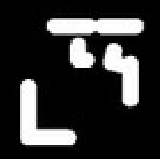
\includegraphics[scale=0.7]{graphics/hinderniskarte.jpg}
\caption{\label{fig:hinderniskarte} Hindernisskarte als Schwarzweiß-Bitmap}
\end{figure}
 In Abbildung \ref{fig:hinderniskarte} ist ein Beispiel eines solches Bitmaps
 zu sehen. Mit der Semantik, dass weiße Areale Hindernisse darstellen und schwarze Bereiche entweder befahrbar
 oder von dieser Position aus nicht einsehbar sind. Diese von uns gewählte Abbildung der Werte
 auf die entsprechenden Bedeutungen ist allerdings beliebig und hat keinen besonderen Grund.
 Die Roboterposition ist der Mittelpunkt der Karte. Bevor Hindernisse in eine solche Karte eingezeichnet werden
 können müssen sie offensichtlich zuvor durch Sensoren detektiert worden sein. Es lag nahe die Laserdaten,
 welche auch zur Lokalisierung eingesetzt und bereits in geeigneter Form vorhanden waren zu nutzen.
 Da ein Roboter in der Realität eine größere Fläche als ein Punkt aufweist entschieden wir uns bereits an dieser
 Stelle zu einer Expansion der Hindernisse auf Robotergröße, damit solche Berechnungen an anderer Stelle vermieden
 werden können.
\missingfigure{MCA2 Obstacle Extractor}
%\begin{figure}[h]
%\center
%\includegraphics[]{}
%\caption{\label{fig:obstacleExtractor} Gruppe \lstinline{Obstacle Extractor}}
%\end{figure}
 In Abbildung \ref{obstacleExtractor} ist die die Gruppe (\lstinline{Obstacle Extractor}),
 durch welche die gewünschte Funktionalität implementiert wurde zu sehen.
 Im Folgenden wollen wir auch hier die einzelnen Module kurz vorstellen:

\todo[inline]{Erläutern der Funktion der Module}

\begin{description}
\item[Modul X] Beschreibung
\item[Modul Y] Beschreibung
\item[Modul Z] Beschreibung
\item[Modul A] Beschreibung
\item[Modul B] Beschreibung
\end{description}
ObstacleExtractor

ci control


SenseIvtErode

ci Erode Mask Size


segwayomnioesmultiplexer
ci control

co Dilate Deactivate Filter
Dilate Mask Size
Erode Deactivate Filter
Erode Mask Size
Update
Sense Update Mode

Hlsp Scan Strategy -> Control
% -----------------------------------------------------------------------------
%													Virtual protective Field
\subsection{Virtual protective Field}
\label{sec:vpf}
Ein Virtual protective Field, was die Letzte von uns zu lösenden Aufgabe darstellte war bereits im Odete-Projekt
 realisiert, allerdings war dieses lediglich für einen Differentialantrieb implementiert.
 Nach einer Begutachtung des bestehenden Moduls entschieden wir uns dafür
 dieses nicht für omnidirektionale Bewegung anzupassen sondern eine neue Gruppe mit der gewünschten Funktionalität
 zu erstellen, da uns dies effizienter erschien. Die Wahl der für die Umsetzung benötigten Primitiven viel, aufgrund
 der von uns gewonnen Erfahrungen mit den Bildverarbeitungs-Modulen und der Möglichkeit die bereits bestehende
 Hinderniskarte auszunutzen auch hier auf die \textcolor{green}{\textbf{SenseIVT}} \todoprivate{ref setzen} Bibliothek.
 Als Repräsentation wurde wieder ein Schwarzweiß-Bitmap gewählt. Auf anfrage der Bahnplanungs und Steuerungs
 Gruppe implementierten wir 3 unterschiedliche Virtual Protective Fields siehe
 Abbildung \ref{fig:virtualprotectivefields}.
 \begin{figure}[h]
\center
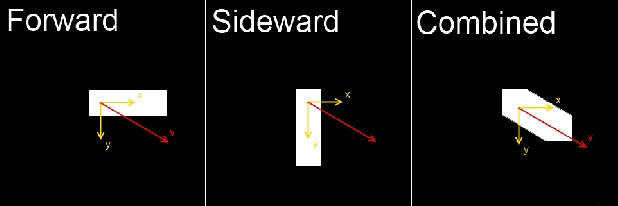
\includegraphics[scale=0.5]{graphics/virtualprotectivefields.jpg}
\caption{\label{fig:virtualprotectivefields} Darstellung der unterschiedlichen Protective
Fields}
\end{figure}
 Die Varianten \emph{Sideward} sowie \emph{Forward} sollen es \gls{hollie}
 ermöglichen eine Bewegung in zumindest eine Richtung durchzuführen wenn die Kombination zu einer Kollision führen würde.
 Die Virtual Protective Fields unterliegen einer dynamischen Ausdehnung zum Quadrat der Geschwindigkeit
 um ein erfolgreiches Anhalten vor einer Kollision zu gewährleisten. Aufgrund der Nutzung von Bildverarbeitungs-Modulen
 konnte die Erkennung einer möglichen Kollision durch eine AND-Operation auf der Hinderniskarte und dem entsprechenden
 Virtual Protective Field realisiert werden. Sollten nach dieser Operation noch weiße Pixel im resultierenden Bitmap
 vorhanden sein gilt dies als erkannte Kollision. Aufgrund von Fehlern der Laserdaten wird verlangt, dass mehr als ein
 weißer Pixel vorhanden ist, um das Verfahren etwas robuster zu machen.
 \missingfigure{MCA2 Virtual Protective Bitmap}
%\begin{figure}[h]
%\center
%\includegraphics[]{}
%\caption{\label{fig:virtualprotectivebitmap} Gruppe \lstinline{Virtual
% Protective Bitmap}}
%\end{figure}
 Wie bereits in den beiden vorigen Abschnitten  ist auch hier in Abbildung \ref{virtualprotectivebitmap}
 die beschriebene Gruppe dargestellt und es folgt eine nähere Betrachtung der Module.
 Wobei wir allerdings nicht erneut näher auf die Module, die bereits zuvor
 vorgestellt wurden eingehen werden.

\todo[inline]{Erläutern der Funktion der Module}

\begin{description}
\item[Modul X] Beschreibung
\item[Modul Y] Beschreibung
\item[Modul Z] Beschreibung
\item[Modul A] Beschreibung
\item[Modul B] Beschreibung
\end{description}
Virtual protective bitmap
Sensor in:
Lateral Velocity
Omni Forward Velocity

controller in:
Control

controller out
Obstacle Forward
Obstacle Sideward
Obstacle Combined

SegwayomnivbpMultiplexer
ci Control
co Update
Sense Update Mode

senseivtandprotectivefield 

ci Deactivate Filter
Last

co Last
Obstacle

sensebitmapsource 
ci Update Source
so Sense Data Type
   Sense Data Changed Counter
   Sense Data Index Left
   Sense Data Index Right

SenseIvtScanToBitmap
ci Deactivate Filter
	Last
co Last

so Sense Data Output Type
   Sense Data Output Counter
   Sense Data Output Left
   Sense Data Output Right
	Last
si Sense Data Input Type
   Sense Data Input Counter
   Sense Data Input Index
   Sense Data Input Right Index
	Last

Parameter
Amount of pixels per mm

Avoidance radius (mm)

SenseIvtProtectiveFieldSource
ci Deactivate Filter
	Last
co Last

so Sense Data Output Type
   Sense Data Output Counter
   Sense Data Output Left
   Sense Data Output Right
	Last
si Sense Data Input Type
   Sense Data Input Counter
   Sense Data Input Index
   Sense Data Input Right Index
	Last
	Velocity
SenseIvtAndProtectiveField
ci Deactivate Filter
	Last
co Last
	Obstacle

so Sense Data Output Type
   Sense Data Output Counter
   Sense Data Output Left
   Sense Data Output Right
	Last
si Sense Data Input Type
   Sense Data Input Counter
   Sense Data Input Index
   Sense Data Input Right Index
	Last